\chapter*{2024年\textsf{HDU}「高等数学2」期中试题解答}

\input{cha/MATH/chapterhead.tex}

\section{选择题（每题3分，共24分）}

\begin{problem}
    过$y$轴与点$(1,2,3)$的平面方程
    \begin{tasks}(4)
        \task $x+y-z=0$
        \task[\true] $3x-z=0$
        \task $2x-y=0$
        \task $3y-2z=0$
    \end{tasks}
\end{problem}
\solute2
\begin{solution}
    取$y$轴上两点$(0,0,0)$，$(0,1,0)$. $\vec S_1=(0,1,0)$，$\vec S_2=(1,2,3)$，$\vec S_1\times\vec S_2=3\vec i-\vec k$，所以$u=(3,0,-1)$. 根据点法式$3(x-1)+0(y-2)-1(z-3)=0$得平面方程为$3x-z=0$.
\end{solution}

\begin{problem}
    设有直线$L_1:\ \frac{x+1}{1}=\frac{y+2}{-2}=\frac{z-4}{1}$与$L_2:\ 
    \begin{cases}
        x-y=6\\
        y-z=3
    \end{cases}$，则$L_1$与$L_2$的夹角为
    \begin{tasks}(4)
        \task $\pi/6$
        \task $\pi/4$
        \task $\pi/3$
        \task[\true] $\pi/2$
    \end{tasks}
\end{problem}
\solute2
\begin{solution}
    $L_2$由两平面相交而成. $\vec n_1=(1,-1,0)$，$\vec n_2=(0,1,-1)$. $\vec S_2=\vec n_1\times\vec n_2=(1,1,1)$. $\vec S_1=(1,-2,1)$. 直线夹角转化为方向向量的夹角$\arccos\braket*[1]{\vec S_1,\vec S_2}=\vec S_1\cdot\vec S_2/\abs*{\vec S_1}\abs*{\vec S_2}=\pi/2$.
\end{solution}

\begin{problem}
    曲线$\begin{cases}
        x=t\\y=t^2\\z=t^3
    \end{cases}$在$t=1$处的切线方程为
    \begin{tasks}(2)
        \task $\frac{x-1}{1}=\frac{y-2}{1}=\frac{z-3}{1}$
        \task[\true] $\frac{x-1}{1}=\frac{y-1}{2}=\frac{z-1}{3}$
        \task $(x-1)+(y-2)+(z-3)=0$
        \task $(x-1)+2(y-1)+3(z-1)=0$
    \end{tasks}
\end{problem}
\solute2
\begin{solution}
    见课本 Page 93 例4.
\end{solution}

\begin{problem}
    设$z=\arcsin\sqrt{1-xy}$，则$\pdv z/x=$
    \begin{tasks}(4)
        \task $\frac{y}{2xy\sqrt{(1-xy)}}$
        \task $\frac{-y}{2xy\sqrt{(1-xy)}}$
        \task $\frac{y}{2\sqrt{xy(1-xy)}}$
        \task[\true] $\frac{-y}{2\sqrt{xy(1-xy)}}$
    \end{tasks}
\end{problem}
\solute2
\begin{solution}
    $z=\arcsin\sqrt{1-xy}$由$z=\arcsin u$，$u=\sqrt v$，$v=\sqrt 1-xy$复合：$z-u-v-x\ \&\ y$.
    $\pdv zx=\odv zu\odv uv\pdv vx=\frac{1}{\sqrt{1-u^2}}\frac12v^{-1/2}(-y)=\frac{-y}{2\sqrt{xy(1-xy)}}$.
\end{solution}

\begin{problem}
    设$z=\e^{\sin(xy)}$，则$\d z=$
    \begin{tasks}(2)
        \task[\true] $\e^{\sin(xy)}\cos(xy)(y\d x+x\d y)$
        \task $\e^{\sin(xy)}\cos(xy)(y+x)$
        \task $\e^{\sin(xy)}(y\d x+x\d y)$
        \task $\e^{\sin(xy)}(y+x)$
    \end{tasks}
\end{problem}
\solute2
\begin{solution}
    $\d z=\pdv zx\d x+\pdv zy\d y=\e^{\sin(xy)}\cos(xy)(y\d x+x\d y)$.
\end{solution}

\begin{problem}
    设$I_1=\iint_D\sqrt{x+y}\d x\d y$，$I_2=\iint_D(x+y)\d x\d y$，$I_3=\iint_D(x+y)^2\d x\d y$，其中$D=\{(x,y)|(x-2)^2+(y-1)^2\leq2\}$，则下列关系成立的是
    \begin{tasks}(4)
        \task $I_1>I_2>I_3$
        \task $I_3>I_1>I_2$
        \task[\true] $I_3>I_2>I_1$
        \task $I_1>I_3>I_2$
    \end{tasks}
\end{problem}
\solute5
\begin{solution}
\begin{paracol}{2}
    由积分区域$D:\ (x-2)^2+(y-1)^2\leq2$可推导出$1\leq x+y$，证明如下.
    \begin{itemize}
        \item 画出积分区域$D$的图像，以$(2,1)$为圆心，$r=\sqrt2$，过点$(1,0)$，$(3,0)$. $d_{\unit{O_1P_1}}=(2+1-1)/\sqrt2=\sqrt2=r$.
        \item 所以$x+y-1=0$与圆相切，积分区域$D$位于$x+y-1=0$上方，所以$x+y-1\geq0$，$x+y\geq1$.
    \end{itemize}
    \switchcolumn
    \begin{figure}[htbp]
        \centering
        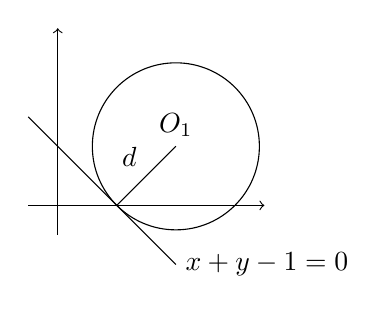
\begin{tikzpicture}[scale=.75]
            \draw [->] (-.5,0) -- (3.5,0);
            \draw [->] (0,-.5) -- (0,3);
            \draw (1,0) -- (2,1) node [above left,midway] {$d$} circle ({sqrt(2)}) node [above] {$O_1$};
            \draw (-.5,1.5) -- (2,-1) node [right] {$x+y-1=0$};
        \end{tikzpicture}
    \end{figure}
    \switchcolumn*[所以$\sqrt{x+y}\leq(x+y)^2\leq(x+y)^3$，$\iint_D\sqrt{x+y}\d x\d y\leq\iint_D(x+y)^2\d x\d y\leq\iint_D(x+y)^3\d x\d y$，所以$I_3>I_2>I_1$.]
\end{paracol}
\end{solution}

\begin{problem}
    设$f(x,y)$是连续函数，$D=\{(x,y)|x^2+y^2\}$，则$\iint_Df(x,y)\d x\d y=$
    \begin{tasks}(2)
        \task[\true] $\int_0^\pi\d\theta\int_0^{\sin\theta}f(\rho\cos\theta,\rho\sin\theta)\rho\d\rho$
        \task $\int_0^\pi\d\theta\int_0^{\cos\theta}f(\rho\cos\theta,\rho\sin\theta)\d\rho$
        \task $2\int_0^1\d y\int_0^{\sqrt{y-y^2}}f(x,y)\d x$
        \task $\int_{-1}^1\d x\int_{-\sqrt{1-x^2}}^{\sqrt{1-x^2}}f(x,y)\d y$
    \end{tasks}
\end{problem}
\solute2
\begin{solution}
    区域可写为$x^2+\ab(y-\frac12)^2\leq\frac14$. $\iint_Df(x,y)\d x\d y=\int_0^\pi\d\theta\int_0^{\sin\theta}f(\rho\cos\theta,\rho\sin\theta)\rho\d\rho$.
\end{solution}

\begin{paracol}{2}
\begin{problem}
    设$f(x,y)$连续，则$\int_0^4\d x\int_{x^2/4}^xf(x,y)\d y=$
    \begin{tasks}(2)
        \task $\displaystyle\int_0^4\d y\int_{2\sqrt y}^yf(x,y)\d x$
        \task $\displaystyle\int_0^4\d y\int_y^1f(x,y)\d x$
        \task $\displaystyle\int_0^4\d y\int_{y^2}^{2\sqrt y}f(x,y)\d x$
        \task[\true] $\displaystyle\int_0^4\d y\int_y^{2\sqrt y}f(x,y)\d x$
    \end{tasks}
\end{problem}
\switchcolumn
\solute3
\begin{solution}
    画出积分区域即可.
    \begin{figure}[htbp]
        \everymath{\scriptstyle}
        \centering
        \begin{tikzpicture}[scale=.4]
            \draw [->] (-.5,0) -- (4.8,0) node [below] {$x$};
            \draw [->] (0,-.5) -- (0,4.8) node [left] {$y$};
            \fill [very thick,pattern=north west lines,variable=\x,domain=0:4,smooth,line cap=round] plot ({\x},{\x*\x/4});
            \draw [very thick,teal,variable=\x,domain=0:4.2,smooth,line cap=round] plot ({\x},{\x*\x/4}) node [left] {$y=x^2/4$};
            \draw [very thick,teal] (-.5,-.5) -- (4.2,4.2) node [right] {$y=x$};
            \draw [dashed] (0,4) node [left] {$4$} -- (4,4) -- (4,0) node [below] {$4$};
        \end{tikzpicture}
    \end{figure}
\end{solution}
\end{paracol}

\section{填空题（每题3分，共12分）}

\begin{problem}
    已知向量$\vec a=2\vec i+\vec j-3\vec k$，则向量$\vec a$在$x$轴上的投影为\ans{$2$}.
\end{problem}
\solute1
\begin{solution}
    $\vec a=2\vec i+\vec j-3\vec k$，向量在$x$轴上的投影为$2$.
\end{solution}

\begin{problem}
    函数$f(x,y,z)=2xy-z^2$在点$(1,-1,1)$处的梯度$\nabla f(1,-1,1)=$\ans{$(-2,2,-2)$}.
\end{problem}
\solute1
\begin{solution}
    $f_x(x,y,z)=2y$，$f_y(x,y,z)=2x$，$f_z(x,y,z)=-2z$. $\nabla f(1,-1,1)=(-2,2,-2)$.
\end{solution}

\begin{problem}
    $\lim\limits_{(x,y)\to(0,0)}\frac{1-\cos(x^2+y^2)}{(x^2+y^2)}=$\ans{$0$}.
\end{problem}
\solute2
\begin{solution}
    $\lim\limits_{(x,y)\to(0,0)}\frac{1-\cos(x^2+y^2)}{(x^2+y^2)}=\lim\limits_{(x,y)\to(0,0)}\frac{(x^2+y^2)^2/2}{(x^2+y^2)}=\lim\limits_{(x,y)\to(0,0)}\frac12(x^2+y^2)=0$.
\end{solution}

\begin{problem}
    设$D=\{(x,y)|x^2+y^2\leq x\}$，则$\iint_D[x^2+y^2+\sin(xy)]\d x\d y=$\ans{$3\pi/32$}.
\end{problem}
\solute2
\begin{solution}
    积分区域可写为$\ab(x-\frac12)^2+y^2\leq\frac14$. $I=\iint_D(x^2+y^2)\d x\d y+\iint_D\sin(xy)\d x\d y=\iint_D(x^2+y^2)\d x\d y=\int_{-\pi/2}^{\pi/2}\d\theta\int_0^{\cos\theta}\rho^2\cdot\rho\d\rho=3\pi/32$.
\end{solution}

\section{计算题 i（每题6分，共24分）}

\begin{problem}
    设$z=u^2\ln v$，而$u=xy$，$v=x+y$，求$\pdv z/x$，$\pdv z/y$.
\end{problem}
\solute4
\begin{solution}\leavevmode
\begin{itemize}
    \item $\pdv zx=\pdv zu\pdv ux+\pdv zv\pdv vx=2u\cdot y\cdot\ln v+u^2\cdot\frac1v\cdot1=2xy^2\ln(x+y)+\frac{x^2y^2}{x+y}$.
    \item $\pdv zy=\pdv zu\pdv uy+\pdv zv\pdv vy=2u\cdot x\cdot\ln v+u^2\cdot\frac1v\cdot1=2x^2y\ln(x+y+\frac{x^2y^2}{x+y})$.
\end{itemize}
\end{solution}

\begin{problem}
    求直线$L:\ 
    \begin{cases}
        x-z+4=0\\x-y+z=0
    \end{cases}$
    在平面$\Pi:\ x-2y-4z+1=0$上的投影直线方程.
\end{problem}
\solute6
\begin{solution}\leavevmode
    \begin{itemize}
        \item 过直线$L$的平面束方程：$x-z+4+\lambda(x-y+z)=0$，即$(1+\lambda)x-\lambda y+(\lambda-1)z+4=0$.
        \item 由此得法向量$\vec n=(1+\lambda,-\lambda,\lambda-1)$. 已知平面法向量$\vec n_0=(1,-2,-4)$，由$\vec n\bot\vec n_0$得$\lambda=5$.
        \item 所以投影直线方程为
        $\begin{cases}
            6x-5y+4z+4=0\\
            x-2y-4z+1=0
        \end{cases}$.
    \end{itemize}
\end{solution}

\begin{problem}
    已知函数$x=x(z)$，$y=y(z)$是由方程组
    $\begin{cases}
        x+y+z=0\\x^2+y^2+z^2=1
    \end{cases}$所确定的函数. 求$\odv x/z$，$\odv y/z$.
\end{problem}
\solute3
\begin{solution}
    方程两边对$z$求导得
    \[\begin{dcases}
        \odv xz+\odv yz+1=0\\
        2x\odv xz+2y\odv yz+2z=0
    \end{dcases}\]
    由此得$\odv x/z=(y-z)/(x-y)$，$\odv y/z=(z-x)/(x-y)$.
\end{solution}

\begin{problem}
    计算$I=\iint_Dxy^2\d x\d y$，其中$D$是圆周$x^2+y^2=4$及$y$轴所围成的右半闭区域.
\end{problem}
\solute3
\begin{solution}\leavevmode
    \begin{itemize}
        \item 直角坐标：$I=\int_{-2}^2\d y\int_0^{\sqrt{4-y^2}}xy^2\d x=\int_{-2}^2\ab[\frac12y^2(4-y^2)]\d y=64/15$.
        \item 或极坐标：$I=\int_{-\pi/2}^{\pi/2}\d\theta\int_0^2\rho^3\cos\theta\sin^2\theta\rho\d\rho=\int_{-\pi/2}^{\pi/2}\cos\theta\sin^2\theta\d\theta\in_0^2\rho^4\d\rho=64/15$.
    \end{itemize}
\end{solution}

\makeatletter
\ifdefstring{\LITE@answer}{hideanswer}{\relax}{\clearpage}
\makeatother

\section{计算题 ii（每题7分，共28分）}

\begin{problem}
    求过点$(2,1,1)$且平行于直线$\frac{x+1}{3}=\frac{y-2}{2}=\frac{z-1}{1}$，又垂直于平面$x+2y+2z-1=0$的平面方程.
\end{problem}
\solute4
\begin{solution}\leavevmode
    \begin{itemize}
        \item 已知直线的方向向量为$\vec s=(3,2,1)$，已知平面的法向量为$\vec n=(1,1,2)$.
        \item 设所求平面法向量$\vec n_0$，则$n_0\bot\vec s$且$\vec n_0\bot\vec n$. 取$\vec n_0=\vec s\times\vec n=(3,-5,1)$.
        \item 所以所求的平面方程为$3(x-2)-5(y-1)+(z-1)=0$. 即$3x-5y+z-2=0$.
    \end{itemize}
\end{solution}

\begin{problem}
    设$z^3-3xyz=a^3$，求$\pdv zx$和$\pdv z{x,y}$.
\end{problem}
\solute4
\begin{solution}\leavevmode
    \begin{itemize}
        \item 令$F(x,y,z)=z^3-3xyz-a^3$，则$F_x=-3yz$，$F_y=-3xz$，$F_z=3z^2-3xy$.
        \item 所以$\pdv zx=-F_z/F_x=yz/(z^2-xy)$，$\pdv zy=-F_y/F_z=xz/(z^2-xy)$.
        \item $\pdv z{x,y}=\frac{\ab(x+y\pdv zy)(x^2-xy)-yz\ab(2z\pdv zy-x)}{(x^2-xy)^2}=\frac{z(z^4-2xyz^2-x^2y^2)}{(x^2-xy)^3}$.
    \end{itemize}
\end{solution}

\begin{problem}
    求上半球体$0\leq z\leq\sqrt{4-(x^2+y^2)}$被圆柱面$x^2+y^2=2x$所截得的（函在圆柱面内的部分）立体的体积.
\end{problem}
\solute2
\begin{solution}
    此立体相当于以$D=\{(x,y)|x^2+y^2\leq2x\}$为底，曲面$z=\sqrt{4-9x^2+y^2}$为顶曲顶柱体. 所以体积
    \[V=\iint_D\sqrt{4-(x^2+y^2)}\d x\d y=\int_{-\pi/2}^{\pi/2}\d\theta\int_0^{2\cos\theta}\sqrt{4-\rho^2}\rho\d\rho=\frac{16}{3}\ab(\frac\pi2-\frac23)\]
\end{solution}

\begin{problem}
    计算二重积分$\iint_D\abs{y-x^2}\d x\d y$，其中$D:\ -1\leq x\leq 1$，$0\leq y\leq1$所确定.
\end{problem}
\solute4
\begin{solution}
    \[\begin{aligned}
        &\iint_D\abs{y-x^2}\d x\d y=\iint_{D_1}(y-x^2)\d x\d y+\iint_{D_2}-(y-x^2)\d x\d\\
        =&\int_{-1}^1\d x\int_{x^2}^1(y-x^2)\d y+\int_{-1}^1\d x\int_0^{x^2}(x^2-y)\d y\\
        =&\int_{-1}^1\ab(\frac12-x^2+\frac12x^4)\d x+\int_{-1}^1\frac12x^4\d x=11/15
    \end{aligned}\]
\end{solution}

\clearpage

\section{综合题（本题8分）}

\begin{problem}
    在球面$x^2+y^2+z^2=\frac12$上求一点$P$，使得函数$f(x,y,z)=x^2+y^2+z^2$在点$P$沿从点$A(1,1,1)$到点$B(2,0,1)$方向点方向导数值最大，并求这个最大值.
\end{problem}
\solute*{\leavevmode\vspace*{\fill}}
\begin{solution}
    因为一个函数沿提督方向点方向导数值最大，所以问题相当于：在球面$x^2+y^2+z^2=\frac12$上求一点$P$，使得函数$f(x,y,z)$在点$P$的梯度$\nabla f(P)$与$\vec{AB}$同向.

    设点$P$的坐标为$(x,y,z)$，函数$f(x,y,z)$在点$P$的梯度$\nabla f(P)=(f_x,f_y,f_z)=2(x,y,z)$，$\vec{AB}=(1,-1,0)$.
    \[\nabla f(P)\parallel\vec{AB},\ \frac x1=\frac{y}{-1}=\frac z0\]
    即$x=-y$，$z=0$. 因为点$P$在球面上，故满足方程$x^2+y^2+z^2=\frac12$. 解得$x_1=\frac12$，$y_1=-\frac12$，$z_1=0$或$x_2=-\frac12$，$y_2=\frac12$，$z_2=0$（后者与$\vec{AB}$反向，舍去）.

    所以函数$f(x,y,z)$在点$\ab(\frac12,-\frac12,0)$沿着点$A$到点$B$得方向导数值最大值为$\abs{\nabla f(P)}=2\sqrt{\ab(\frac12)^2+\ab(-\frac12)^2+0}=\sqrt2$.
\end{solution}

\begin{problem}
    设函数$f(x)$在$[a,b]$上连续，且$f(x)>0$，证明不等式
    \[\int_a^bf(x)\d x\cdot\int_a^b\frac{1}{f(x)}\d x\geq(b-a)^2\]
\end{problem}
\solute*{\leavevmode\vspace*{\fill}}
\begin{solution}
\begin{proof}
    记区域$D=\{(x,y)|a\leq x\leq b,a\leq y\leq b\}$，则
    \[\begin{aligned}
        \text{LHS}&=\int_a^bf(x)\d x\cdot\int_a^b\frac{1}{f(y)}\d y=\iint_D\frac{f(x)}{f(y)}\d x\d y=\iint_D\frac{f(y)}{f(x)}\d x\d y\\
        &=\frac12\ab[\iint_D\frac{f(x)}{f(y)}\d x\d y+\iint_D\frac{f(y)}{f(x)}\d x\d y]=\frac12\iint_D\ab[\frac{f(x)}{f(y)}+\frac{f(y)}{f(x)}]\d x\d y\\
        &\geq\frac12\iint_D2\d x\d y=(b-a)^2
    \end{aligned}\]
    所以不等式成立.
\end{proof}
\end{solution}